\chapter[Wstęp ]{Wstęp}
Szybki postęp technologiczny zapoczątkowany w XX wieku umożliwił rozwój nowych dziedziń nauki, między innymi robotyki. Obecnie maszyny mogą zastępować ludzi przy wykonywaniu wielu rozmaitych czynności.
Innowacyjne rozwiązania stwarzają jednak potrzebę opracowania wymagającego środowiska testowego. Jedną z takich inicjatyw, mających na celu wspieranie rozwoju i popularyzację robotyki są rozgrywki
RoboCup. W obrębie przedsięwzięcia wyróżnionych jest kilka lig, różniących się zasadami oraz typem robotów biorących udział w zawodach.
Głównym celem przyświecającym organizatorom jest stworzenie do 2050 roku drużyny robotów zdolnej wygrać z ówczesnymi mistrzami świata.
Liga RoboCup budzi zainteresowanie wielu ludzi na całym świecie, prace z nią związane  są prowadzone w wielu środowiskach akademickich na całym świecie.
W Polsce nie została jeszcze stworzona drużyna, która wystartowałaby w tych rozgrywkach.
Rozwiązanie problemu stawia przed uczestnikami wyzwania konstukcyjne oraz algorytmiczne. Niniejsza praca skupiona jest głównie na rowiązaniach algorytmicznych. Omówniony zostanie problem sterowania
zawodnikiem, wyznaczania bezkolizyjnej ścieżki do celu oraz reazlizacji prostych zachowań niezbędnych podczas rozgrywek.
\section{Zakres pracy}
Niniejsza praca jest niejako kontynuacją działań podjętych podczas realizacji pracy inżynierskiej. Tematyka w niej poruszona dotyczy na wstępie samych rozgrywek RoboCup. Jak już napisano we 
wstępie przedsięwzięcie dotyczny głównie rogrywek piłkarkich, w których udział biorą roboty. Jednak ze względu na dynamiczny rozwój samej robotyki do projektu dołączane są kolejne tematy.
Obecnie podział jest następujący:
\begin{itemize}
	\item \emph{RoboCupSoccer}, czyli rozgrywki piłkarskie autonomicznych robotów,
	\item \emph{RoboCupRescue}, obejmujący działania robotów w sytuacjach kryzysowych, czy niebezpiecznych dla ludzi,
	\item \emph{RoboCup@Home}, skupiający się na robotyce mającej na celu pomaganie człowiekowi w codziennych czynnościach,
	\item \emph{RoboCupJunior} popularyzujący robotykę wśród młodzieży.
\end{itemize}

Same rozgrywki piłkarskie \emph{RoboCupSoccer} także są podzielone na kilka lig, tutaj głównym kryterium jest konstrukcja mechaniczna zawodników. Więcej informacji na ten temat zostanie zaprezentowanych w rozdziale
\ref{chap:robocup}. W ramach samej pracy skupiono się na lidze małych robotów (\emph{Small-size League}), ponieważ już wcześniej prowadzone były prace w tym kierunku na Wydziale Elektroniki i 
Technik Informacyjnych Politechniki Warszawskiej.

W dalszej części pracy opisano nowe testowe środowisko symulacyjne oraz wprowadzone poprawki modyfikujące pracę symulatora.
Z racji, iż wczesniejsze prace prowadzono na symulatorze \emph{Player/Stage/Gazebo} zdecydowano się na dalsze prace na tej platformie.
Opracowane zostały nowe modele zawodników, wzorowane na rzeczywistych, holonomicznych
biorących udział w rozgrywkach. Opracowano sterownik (element symulatora) umożliwiający: kontrolę nad prędkością robota (wyposażono go dodatkowo w regulator PID), prowadzenie piłki jak i oddawanie strzału.
 W stosunku do poprzednich prac zdecydowano się także na implementację oraz poddanie testom nowego algorytmu nawigacji.  Rozwiązanie to zostało przetestowane w takich samych warunkach 
jak poprzednie. Dokonano także analizy i porównania otrzymanych wyników. Zaprezentowano także inne, stosowane w robotyce metody unikania kolizji. Jeden z nich także został zaimplementowany, w celu
rozwiązywania mniej złożonych zadań, takich jak odjechanie od przeszkody w momencie wystąpienia kolizji.

W pracy zostało przedstawione także jedno z podejść, powszechnie stosowane do koordynacji i planowania działań zawodników (\mbox{\texttt{STP - Skill Tactics Play}} \cite{stp}).
Zakłada ono planowanie zachowań drużyny na $3$ poziomach. Każdy odnosi się do innej warstwy abstrakcji.
\begin{enumerate} 
  \item Poziomem najwyżej w hierachii jest \texttt{Play}. Przez to pojęcie rozumiany jest plan gry dla całej drużyny, uwzględniana jest tutaj koordynacja
  poczynań pomiędzy zawodnikami. Plan zakłada przydział zawodnika do określonej roli. W oryginalnym rozwiązaniu role przydzielane są dynamicznie w zależności od sytuacji na boisku.
  W obrębie danego planu zawodnik wykonuje swoją rolę (sekwencję kilku \texttt{Tactics}), aż do momentu zakończenia danego planu lub wyznaczenia kolejnego.
  
  \item Przez \texttt{Tactics} rozumiany jest plan działań dla jednej roli. W taktyce zamknięte jest wykonywanie przez robota pojedynczej złożonej akcji.
  Przykładem może być strzał na bramkę. Robot dostaje polecenie oddania strzału na bramkę, zatem plan jego poczynań ma doprowadzić
 do sytuacji, w której osiągnie on pozycję umożliwiającą odddanie strzału na bramkę z zadanym powodzeniem.
 Plan na szczeblu pojedynczego robota jest wykonywany do momentu zmiany planu gry całej drużyny (ponownego przydziału robotów do ról).
 Przykładowe \texttt{Tactics}:
 \begin{itemize}
  \item strzał na bramkę,
  \item podanie piłki,
  \item odebranie podania,
  \item blokowanie innego robota,
  \item wyjście na pozycję,
  \item bronienie pozycji,
  \item dryblowanie z piłką.
 \end{itemize}
  Taktyka determinuje skończony automat stanów, w którym elementami są \texttt{Skills}. Wykonanie bieżącej taktyki sprwadza się do przechodzenia pomiędzy kolejnymi zachowaniami robota w obrębie
  danego automatu.
  \item Najniżej w hierarchii znajduje się pojęcie \texttt{Skills} odnosi się ono do konkretnych umiejętności robota, takich jak:
    \begin{itemize}
    \item przechwycenie piłki,
    \item oddanie strzału,
    \item doprowadzenie piłki do celu,
    \item przemieszczenie robota do celu,
    \item podążanie za innym robotem.
    \end{itemize}
  Na tym szczeblu nie wystąpuje koordynacja w obrębie drużyny. Zachowanie robota zmieniane jest w każdym kroku gry. Z każdego \texttt{Skill}, w każdym momencie określone musi być przejście
  albo do nowego zadania bądź kontynuowanie tego samego zadania. Przykładowo jeśli zlecimy robotowi przemieszczenie z piłką do celu i piłka 
  odskoczy robotowi, to powinien do niej podjechać, przechwycić ją, a następnie ponownie prowadzić do zadanego celu (należy jednak cały czas pamiętać, że jeśli nastąpi dobra okazja do strzału
na bramkę to należy z niej skorzysta.
\end{enumerate}

 W ramach pracy w pełni zrealizowane zostały dwie warstwy z oryginalnej hierarchii opisanej powyżej (\texttt{Skills} oraz \texttt{Tactics}). Aplikację projektowano w taki sposób, aby pozostawić miejsce
 na implementację warstwy \texttt{Play}, której niedkończono.
Użyteczność algorytmu sprawdzono podczas przeprowadzonych eksperymentów, wzorowanych na rzeczywistych zadaniach eliminacyjnych stosowanych w rozgrywkach RoboCup w ostatnich latach.

\section{Cel pracy}
Za główny cel niniejszej pracy postawiono przetestowanie użyteczności i skuteczności architektury \texttt{STP}. Aby jednak zrealizować to zadanie konieczne było
stworzenie środowiska symulacyjnego, umożliwiającego modelowanie rozgrywki \emph{Small-size League}. Przy opracowywaniu modelu środowiska starano się w jak największym stopniu odzwierciedlić realia
ligi \emph{Small-size League}. Po drugie środowisko symulacyjne miało być na tyle elastyczne, aby w przyszłości umożliwiało testowanie różnorodnych rozwiązań sterowania drużyną.
Zachowano schemat przepływu informacji z pracy inżynierskiej. Został on zamieszczony na rysunku \ref{fig:przeplyw_sterowania}. Stosowany w rozgrywach \emph{Small-size League} \texttt{videoserwer} został
zamodelowany jako osobna warstwa  aplikacji, komunikująca się bezpośrednio z symulatorem. Osobną warstwę stanowi także część aplikacji odpowiedzialna za sterowanie robotem.
\begin{figure}[H]
\centering
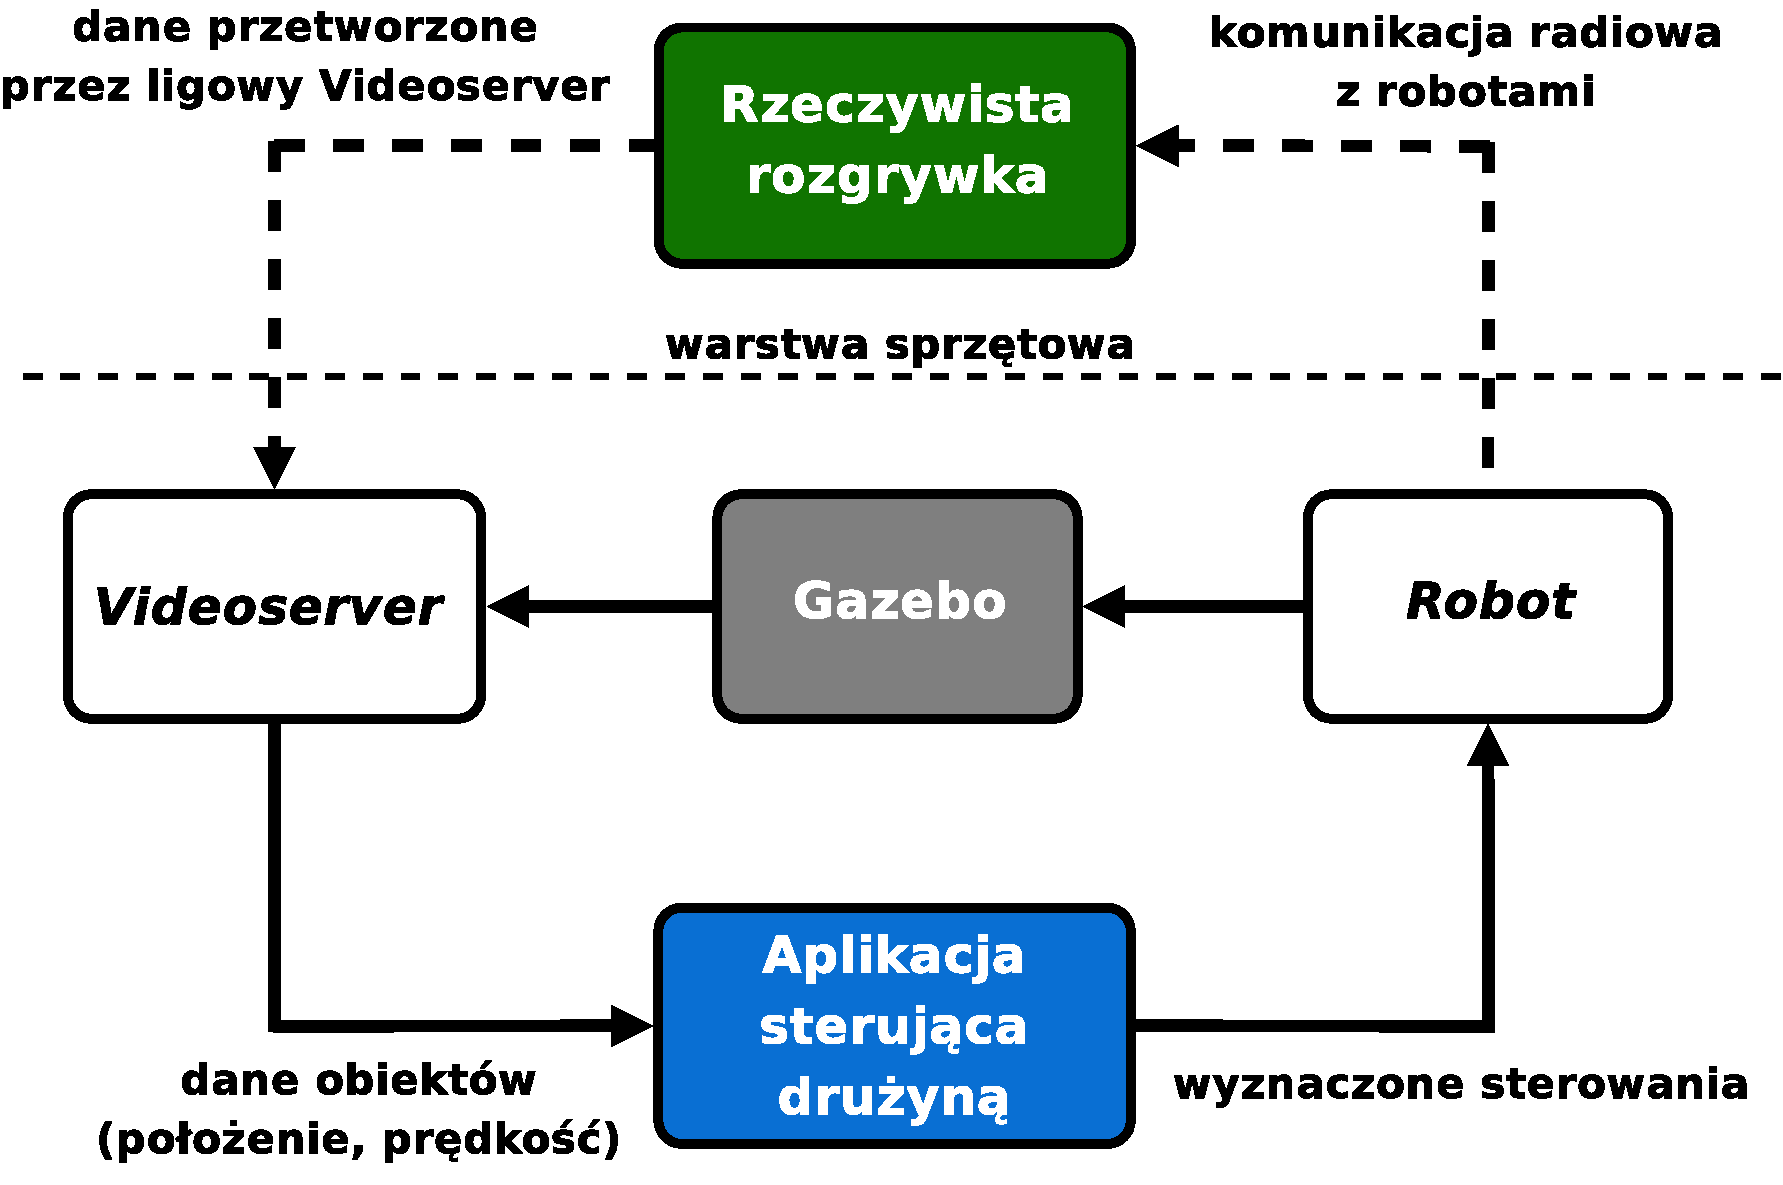
\includegraphics[scale=0.38]{./zalozenia/przeplyw_sterowania.pdf}
\caption{Komunikacja pomiędzy warstwami aplikacji.} \label{fig:przeplyw_sterowania}
\end{figure}
Główną motywacją takiej architektury było umożliwienie prostego przystosowania aplikacji do sterowania rzeczywistym robotem pobierającym dane z zewnętrznego serwera. 
Ponieważ w rozgrywkach biorą udział roboty holonomiczne, zdecydowano się na odejście od modelu robota o napędzie różnicowym stosowanego w pracy inżynierskiej (wzorowanego na \textit{HMT}) i opracowanie nowego wzorowanego na rzeczywistych
zawodnikach.
Kolejnym celem pracy wynikającym bezpośrednio ze zmiany modelu zawodnika, było zaimplementowanie i przetestowanie algorytmu nawigacji robota w dynamicznym środowisku. Zdecydowano się na algorytm \texttt{RRT},
postanowiono także porównać jego skuteczność z wcześniej stosowanym \texttt{CVM}.

